\ifdefined\included
\else
\documentclass[a4paper,11pt,twoside]{StyleThese}
\usepackage{amsmath,amssymb, amsthm}             % AMS Math
\usepackage[T1]{fontenc}
\usepackage[utf8x]{inputenc}
\usepackage{babel}
\usepackage{datetime}

\usepackage{silence}

\WarningFilter{minitoc(hints)}{W0023}
\WarningFilter{minitoc(hints)}{W0028}
\WarningFilter{minitoc(hints)}{W0030}

\usepackage{lmodern}
\usepackage{tabularx}
%\usepackage{tabular}
\usepackage{multirow}
\usepackage{xspace}

\usepackage{subfig}
\usepackage[inline]{enumitem}

\usepackage{hhline}
\usepackage[left=1.5in,right=1.3in,top=1.1in,bottom=1.1in,includefoot,includehead,headheight=13.6pt]{geometry}
\renewcommand{\baselinestretch}{1.05}

% Table of contents for each chapter

\usepackage[nottoc, notlof, notlot]{tocbibind}
\usepackage{minitoc}
\setcounter{minitocdepth}{2}
\mtcindent=15pt
% Use \minitoc where to put a table of contents

\usepackage{aecompl}

% Glossary / list of abbreviations

\usepackage[intoc]{nomencl}
\iftoggle{ThesisInEnglish}{%
\renewcommand{\nomname}{Glossary}
}{ %
\renewcommand{\nomname}{Liste des Abréviations}
}

\usepackage{etoolbox}
\renewcommand\nomgroup[1]{%
  \item[\bfseries
  \ifstrequal{#1}{A}{Number Sets}{%
  \ifstrequal{#1}{G}{Agents Beliefs and Action Models}{%
  \ifstrequal{#1}{N}{Navigation}{%
  \ifstrequal{#1}{O}{Ontology}{%
  \ifstrequal{#1}{R}{Referring Expression Generation}{%
  \ifstrequal{#1}{Z}{Controllable and Uncontrollable Agents Task Planning}{}}}}}}%
]}

\makenomenclature



% My pdf code

\usepackage{ifpdf}

\ifpdf
  \usepackage[pdftex]{graphicx}
  \DeclareGraphicsExtensions{.jpg}
  \usepackage[pagebackref,hyperindex=true]{hyperref}
  \usepackage{tikz}
  \usetikzlibrary{arrows,shapes,calc}
\else
  \usepackage{graphicx}
  \DeclareGraphicsExtensions{.ps,.eps}
  \usepackage[dvipdfm,pagebackref,hyperindex=true]{hyperref}
\fi

\graphicspath{{.}{images/}}

%% nicer backref links. NOTE: The flag ThesisInEnglish is used to define the
% language in the back references. Read more about it in These.tex

\iftoggle{ThesisInEnglish}{%
\renewcommand*{\backref}[1]{}
\renewcommand*{\backrefalt}[4]{%
\ifcase #1 %
(Not cited.)%
\or
(Cited in page~#2.)%
\else
(Cited in pages~#2.)%
\fi}
\renewcommand*{\backrefsep}{, }
\renewcommand*{\backreftwosep}{ and~}
\renewcommand*{\backreflastsep}{ and~}
}{%
\renewcommand*{\backref}[1]{}
\renewcommand*{\backrefalt}[4]{%
\ifcase #1 %
(Non cité.)%
\or
(Cité en page~#2.)%
\else
(Cité en pages~#2.)%
\fi}
\renewcommand*{\backrefsep}{, }
\renewcommand*{\backreftwosep}{ et~}
\renewcommand*{\backreflastsep}{ et~}
}

% Links in pdf
\usepackage{color}
\definecolor{linkcol}{rgb}{0,0,0.4} 
\definecolor{citecol}{rgb}{0.5,0,0} 
\definecolor{linkcol}{rgb}{0,0,0} 
\definecolor{citecol}{rgb}{0,0,0}
% Change this to change the informations included in the pdf file

\hypersetup
{
bookmarksopen=true,
pdftitle="Endowing the robot with the abilities to control and evaluate its contribution to a human-robot joint action",
pdfauthor="Amandine MAYIMA", %auteur du document
pdfsubject="Thèse", %sujet du document
%pdftoolbar=false, %barre d'outils non visible
pdfmenubar=true, %barre de menu visible
pdfhighlight=/O, %effet d'un clic sur un lien hypertexte
colorlinks=true, %couleurs sur les liens hypertextes
pdfpagemode=None, %aucun mode de page
pdfpagelayout=SinglePage, %ouverture en simple page
pdffitwindow=true, %pages ouvertes entierement dans toute la fenetre
linkcolor=linkcol, %couleur des liens hypertextes internes
citecolor=citecol, %couleur des liens pour les citations
urlcolor=linkcol %couleur des liens pour les url
}

% definitions.
% -------------------

\setcounter{secnumdepth}{3}
\setcounter{tocdepth}{2}

% Some useful commands and shortcut for maths:  partial derivative and stuff

\newcommand{\pd}[2]{\frac{\partial #1}{\partial #2}}
\def\abs{\operatorname{abs}}
\def\argmax{\operatornamewithlimits{arg\,max}}
\def\argmin{\operatornamewithlimits{arg\,min}}
\def\diag{\operatorname{Diag}}
\newcommand{\eqRef}[1]{(\ref{#1})}

\usepackage{rotating}                    % Sideways of figures & tables
%\usepackage{bibunits}
%\usepackage[sectionbib]{chapterbib}          % Cross-reference package (Natural BiB)
%\usepackage{natbib}                  % Put References at the end of each chapter
                                         % Do not put 'sectionbib' option here.
                                         % Sectionbib option in 'natbib' will do.
\usepackage{fancyhdr}                    % Fancy Header and Footer

% \usepackage{txfonts}                     % Public Times New Roman text & math font
  
%%% Fancy Header %%%%%%%%%%%%%%%%%%%%%%%%%%%%%%%%%%%%%%%%%%%%%%%%%%%%%%%%%%%%%%%%%%
% Fancy Header Style Options

\pagestyle{fancy}                       % Sets fancy header and footer
\fancyfoot{}                            % Delete current footer settings

%\renewcommand{\chaptermark}[1]{         % Lower Case Chapter marker style
%  \markboth{\chaptername\ \thechapter.\ #1}}{}} %

%\renewcommand{\sectionmark}[1]{         % Lower case Section marker style
%  \markright{\thesection.\ #1}}         %

\fancyhead[LE,RO]{\bfseries\thepage}    % Page number (boldface) in left on even
% pages and right on odd pages
\fancyhead[RE]{\bfseries\nouppercase{\leftmark}}      % Chapter in the right on even pages
\fancyhead[LO]{\bfseries\nouppercase{\rightmark}}     % Section in the left on odd pages

\let\headruleORIG\headrule
\renewcommand{\headrule}{\color{black} \headruleORIG}
\renewcommand{\headrulewidth}{1.0pt}
\usepackage{colortbl}
\arrayrulecolor{black}

\fancypagestyle{plain}{
  \fancyhead{}
  \fancyfoot{}
  \renewcommand{\headrulewidth}{0pt}
}

%\usepackage{MyAlgorithm}
%\usepackage[noend]{MyAlgorithmic}
\usepackage{algorithm}
\usepackage[noend]{algpseudocode}
\usepackage{comment}
\usepackage[ED=MITT-InfoTel, Ets=INSA]{tlsflyleaf}
%%% Clear Header %%%%%%%%%%%%%%%%%%%%%%%%%%%%%%%%%%%%%%%%%%%%%%%%%%%%%%%%%%%%%%%%%%
% Clear Header Style on the Last Empty Odd pages
\makeatletter

\def\cleardoublepage{\clearpage\if@twoside \ifodd\c@page\else%
  \hbox{}%
  \thispagestyle{empty}%              % Empty header styles
  \newpage%
  \if@twocolumn\hbox{}\newpage\fi\fi\fi}

\newcommand*{\algrule}[1][\algorithmicindent]{%
	\makebox[#1][l]{%
		\hspace*{.2em}% <------------- This is where the rule starts from
		\vrule height .75\baselineskip depth .25\baselineskip
	}
}

%%% to have lines in algorithm, from stackexchange
\newcount\ALG@printindent@tempcnta
\def\ALG@printindent{%
	\ifnum \theALG@nested>0% is there anything to print
	\ifx\ALG@text\ALG@x@notext% is this an end group without any text?
	% do nothing
	\else
	\unskip
	% draw a rule for each indent level
	\ALG@printindent@tempcnta=1
	\loop
	\algrule[\csname ALG@ind@\the\ALG@printindent@tempcnta\endcsname]%
	\advance \ALG@printindent@tempcnta 1
	\ifnum \ALG@printindent@tempcnta<\numexpr\theALG@nested+1\relax
	\repeat
	\fi
	\fi
}
% the following line injects our new indent handling code in place of the default spacing
\patchcmd{\ALG@doentity}{\noindent\hskip\ALG@tlm}{\ALG@printindent}{}{\errmessage{failed to patch}}
\patchcmd{\ALG@doentity}{\item[]\nointerlineskip}{}{}{} % no spurious vertical space
% end vertical rule patch for algorithmicx

\makeatother
 
%%%%%%%%%%%%%%%%%%%%%%%%%%%%%%%%%%%%%%%%%%%%%%%%%%%%%%%%%%%%%%%%%%%%%%%%%%%%%%% 
% Prints your review date and 'Draft Version' (From Josullvn, CS, CMU)
\newcommand{\reviewtimetoday}[2]{\special{!userdict begin
    /bop-hook{gsave 20 710 translate 45 rotate 0.8 setgray
      /Times-Roman findfont 12 scalefont setfont 0 0   moveto (#1) show
      0 -12 moveto (#2) show grestore}def end}}
% You can turn on or off this option.
% \reviewtimetoday{\today}{Draft Version}
%%%%%%%%%%%%%%%%%%%%%%%%%%%%%%%%%%%%%%%%%%%%%%%%%%%%%%%%%%%%%%%%%%%%%%%%%%%%%%% 

\newenvironment{maxime}[1]
{
\vspace*{0cm}
\hfill
\begin{minipage}{0.5\textwidth}%
%\rule[0.5ex]{\textwidth}{0.1mm}\\%
\hrulefill $\:$ {\bf #1}\\
%\vspace*{-0.25cm}
\it 
}%
{%

\hrulefill
\vspace*{0.5cm}%
\end{minipage}
}

\let\minitocORIG\minitoc
\renewcommand{\minitoc}{\minitocORIG \vspace{1.5em}}

\usepackage{multirow}
%\usepackage{slashbox}

\newenvironment{bulletList}%
{ \begin{list}%
	{\tiny$\bullet$}%
	{\setlength{\labelwidth}{25pt}%
	 \setlength{\leftmargin}{30pt}%
	 \setlength{\itemsep}{-0.5em}}}%
{ \end{list} }

\newenvironment{inlineEnumerate}
{\begin{enumerate*} [label={(\arabic*)}] }
{\end{enumerate*}}

\theoremstyle{definition}
\newtheorem{definition}{Definition}
\renewcommand{\epsilon}{\varepsilon}

% centered page environment

\newenvironment{vcenterpage}
{\newpage\vspace*{\fill}\thispagestyle{empty}\renewcommand{\headrulewidth}{0pt}}
{\vspace*{\fill}}

\newenvironment{asl}{\ttfamily\begin{tabbing}~~~\=$\leftarrow$ \= ~~~ \=
		\kill}{\end{tabbing}}

\usepackage{tablefootnote}

\theoremstyle{plain}
\newtheorem{constraint}{Constraint}[section]

\algnewcommand\algorithmicforeach{\textbf{for each}}
\algnewcommand\algorithmicin{\textbf{in}}
\algdef{S}[FOR]{ForEach}[2]{\algorithmicforeach\ #1\ \algorithmicin\ #2\ \algorithmicdo}

\algnewcommand\algorithmicforkxor{\textbf{do fork-join-xor}}
\algnewcommand\algorithmicendforkxor{\textbf{end fork-join-xor}}
\algdef{SE}{ForkXor}{EndForkXor}{\algorithmicforkxor}{\algorithmicendforkxor}


\usepackage{listings}
\lstset{
	frame=single,
	captionpos=b,
	breaklines=true,
	basicstyle=\ttfamily,
	numberstyle=\color{black},
	tabsize=2,
	mathescape=true,
	literate=%
		{â}{{\^a}}1
}

\lstdefinestyle{inline}{
	frame=none,
	aboveskip=\smallskipamount,
	belowskip=\smallskipamount,
}

\lstdefinestyle{OwlTurtle}{
	language=C,
	tabsize=4,
	basicstyle=\scriptsize\ttfamily,
	keywordstyle=\bfseries\color{darkgray},
	morekeywords={rdf:type, rdfs:domain, rdfs:subPropertyOf, rdfs:range, :hasSubtask, :DecompositionUsedBy, rdfs:subClassOf, :hasDecomposition, owl:inverseOf, htn_actions:hasEffect, rdfs:label},
	alsoletter=:
}

\lstdefinestyle{aslDef}{
	frame=none,
%	breaklines=false,
	%xleftmargin=.1\textwidth, xrightmargin=.1\textwidth
}

\fancypagestyle{example}{%
	\fancyhead[LE]{\bfseries\thepage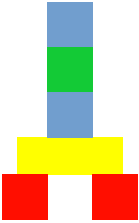
\includegraphics[scale=0.20]{figures/chapter2/task_goal.pdf}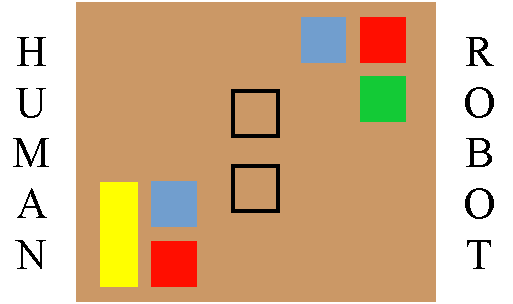
\includegraphics[scale=0.18]{figures/chapter2/task_setup_mini.pdf}}   
	\fancyhead[RO]{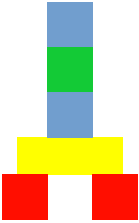
\includegraphics[scale=0.20]{figures/chapter2/task_goal.pdf}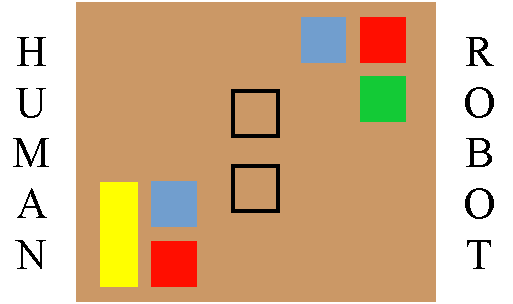
\includegraphics[scale=0.18]{figures/chapter2/task_setup_mini.pdf}\bfseries\thepage}  
	\fancyhead[RE]{\bfseries\nouppercase{\leftmark}}      % Chapter in the right on even pages
	\fancyhead[LO]{\bfseries\nouppercase{\rightmark}}     % Section in the left on odd pages
}%

\usepackage{pdfpages}
\usepackage{makecell}
\usepackage{pdflscape} 
\usepackage{mathtools}
\usepackage[section]{placeins}
\usepackage{afterpage}

%%%%%%%% my commands
\newcommand{\etal}{\textit{et al}.}
\newcommand{\ie}{\textit{i.e.}, }
\newcommand{\eg}{\textit{e.g.}, }
\newcommand{\fact}[3]{\mbox{\textit{#1}(#2, #3)}}
\newcommand{\circledtext}[1]{\raisebox{.5pt}{\textcircled{\raisebox{-.9pt} {#1}}}}
\newcommand{\sparql}{\textsc{SPARQL}}

\newcommand{\algConst}[1]{${\scriptscriptstyle #1}$}
\newcommand{\algNormTextSub}[2]{$\text{#1}_{#2}$}

\newcommand{\aslnumber}[1]{$#1$}
\newcommand{\aslstring}[1]{\textsf{#1}}
\newcommand{\aslvar}[1]{\textcolor{purple}{\textit{#1}}}
\newcommand{\asllabel}[1]{\textbf{#1}}
\newcommand{\annotation}[1]{{\footnotesize #1}}
\newcommand{\rulebody}[1]{\mbox{\hspace{.05\linewidth}}\begin{minipage}[t]{0.9\linewidth}#1.\end{minipage}}
\newcommand{\context}[1]{\begin{minipage}[t]{0.9\linewidth}#1\end{minipage}}
\newcommand{\planbody}[1]{\begin{minipage}[t]{0.9\linewidth}#1.\end{minipage}}
\newcommand{\Jason}[0]{\textbf{\textit{Jason}}}
\newcommand{\sn}{\mbox{\large\textbf{\texttt{\textasciitilde}}}}


\sloppy
\begin{document}
	\setcounter{chapter}{4} %% Numéro du chapitre précédent ;)
	\dominitoc
	\faketableofcontents
	\fi

\chapter{JAHRVIS by the menu}
\label{chapter:chap2}
\minitoc

%\chapter{Joint Action-based Human-Aware supeRVISor: JAHRVIS}
%\label{chapter:chap2}
%\chaptermark{JAHRVIS}
%\minitoc

In the previous chapter, we presented all the previous works we got our inspiration from, from psychology to robotics by way of philosophy, sociology and neuroscience. What is a social interaction? how can it be divided in steps? what is a joint action? how humans collaborate together? how do they take into account their partners? what happens when an agent makes a mistake? what has been done in computer science or robotics until now to make robots better collaborators? All these theories, ideas, questionings nourished our thoughts for the design and implementation of a supervision system dedicated to Human-Robot Joint Action. Supervision is key in the architecture as it is the robot decision kernel. And, as most components of a robotic architecture dedicated to \acrshort{hri}, one of the main issues of supervision is how to take the human into account, a more or less unpredictable agent with whom the robot has to collaborate. 

We presented in Section~\ref{chap1:subsec:state_art_sup} a few works tackling supervision issues, \ie how to adapt to the human, how to monitor them, how to face unexpected human behavior, how to optimize the task efficiency, how to make the robot an good human helper... They were very inspiring but we thought it was missing a general architecture and a software that could be used in different types of collaborative tasks, available for the community and that could easily be enhanced with new features. These thoughts led to the development of the \acrfull{jahrvis} which is the central topic of this chapter. We also came up with a novel idea: to endow the robot with the ability to measure if an interaction is going well or not. Such ability can be used by the supervision to enhance its adaptation capacity.

In the two first sections, we present the role and features we defined for \acrshort{jahrvis}. Next, in Section~\ref{chap5:sec:levels}, we present our representation of Human-Robot collaborative activity. Finally, we introduce \acrshort{jahrvis} overall structure in Section~\ref{chap5:sec:jahrvis} whose role is to decide and control the robot during an interaction.

\section{The Role and Features of JAHRVIS}\label{chap5:sec:sup_features}

\acrshort{jahrvis} is a supervision system, \ie it embeds the robot high-level decisions, controls its behavior and tries to react to contingencies, whenever necessary considering the human the robot is interacting with. Thus, \acrshort{jahrvis} is to differentiate from supervision systems dedicated to robot or multi-robots control as humans are taken into account. 

It queries, manages and executes (shared) plans which are (partially) ordered set of actions to be performed by human and robot agents in order to achieve a (shared) goal. The plan management, described in Section~\ref{chap6:sec:plan_handling}, is based on the estimation of the human's mental states, its knowledge about the current state of the environment, and recognized human actions. We explored the management of various kind of plans: 
\begin{inlineEnumerate}
	\item shared plans in which each action is allocated to an agent as well as action parameters are given objects,
	\item shared plans in which actions might not be allocated to an agent at planning time and parameters might refer to objects with a semantic query, and
	\item conditional plans which anticipate different possibilities for the human decision/action. 
\end{inlineEnumerate} 

As mentioned previously, the plan management relies on the recognition of human actions, among other things. \acrshort{jahrvis} integrates its own processes of action monitoring, \ie selecting the robot's point of interest and enabling joint attention, presented in Sections~\ref{chap6:subsec:robot_plan} and \ref{chap6:para:resource_m}, and of action recognition. This latter process, introduced in Section~\ref{chap6:sec:h_moni}, is model-based and have been designed to be robust to a potentially unreliable perception of the human.

As there are actions of the plan to execute by the robot, \acrshort{jahrvis} needs interfaces with the robot controllers. Moreover, actions can be of two types, physical and communicative actions, and so requires a differentiated management. The methods implemented to handle the action execution will be introduced in Section~\ref{chap6:sec:aem}.

Finally, an important feature is the ability to verbally communicate with the human. Indeed, during a collaborative task, communicate might be needed, among other things, to inform the partner of a performed action, or to ask them to perform one. Section~\ref{chap6:sec:comm} describes the choices we made to endow the robot with a minimum set of communication abilities.

%Not only \acrshort{jahrvis} controls the robot contribution to a collaborative task, it also tries to evaluate if the interaction is going well or not. It is possible thanks to a set of metrics we have built and a method to aggregate them. We claim that having a robot with this ability allows it to enhance and make its decision-making processes more pertinent. The evaluation of the \acrlong{qoi} relies on a model of interaction, considered at  three levels: the interaction session level, the tasks level and the actions level. In future work, this granularity will allow the robot to know precisely on what level it needs to act when a low \acrshort{qoi} is assessed. Indeed, for instance, a task can be of poor quality while the session can still be considered as going well. \acrshort{qoi} principles and metrics will be described in Chapter~\ref{chapter:chap7}.




\section{Representation of a Human-Robot collaborative activity}\label{chap5:sec:levels}
It is possible to describe and decompose a Human-Robot collaborative/joint activity in various ways for (see Section~\ref{chap1:subsec:def_ja} for discussions related to joint or collaborative activities). What we define as collaborative activities or tasks are types of joint actions. For all the following definitions, we place ourselves in the context of one-to-one human-robot interactions, however we  believe that the scheme can be extended to multi-human multi-robot contexts. 
We draw our inspiration from the literature of sociology and robotics, presented in Section~\ref{chap1:sec:soc_int} and Section~\ref{chap2:sec:soc_inter}, to define a model of interaction with three layered levels: interaction session, tasks and actions; as illustrated in Fig.~\ref{fig:levels}. We chose to represent collaborative tasks and their decomposition using the \acrfull{htn}~\cite{ghallab_2016_automated} representation which is often used in cognitive robotics~\cite{ingrand-2017,lallement_2014_hatp, buisan_2021_human} and because it allows to deal with goal-based and situation-based activities at different levels of hierarchy such as task, subtasks and actions and consequently to consider different levels of granularity. 

%In the example of a task with an overall bad Quality of Interaction, it would be interesting to know that in fact it is only a particular action or subtask ruining it. Indeed, the other parts of the task can be ok, or on the opposite, a particular subtask or action can have performed very well among the others. We need and use this granularity also on the three levels defined (interaction session, tasks and actions) to finely evaluate the Quality of Interaction, as a task can be of poor quality but the session is globally going well, \eg if a given task was a complete failed for some reasons but the other tasks were performed correctly. 

\begin{figure}[!ht]
	\centering
	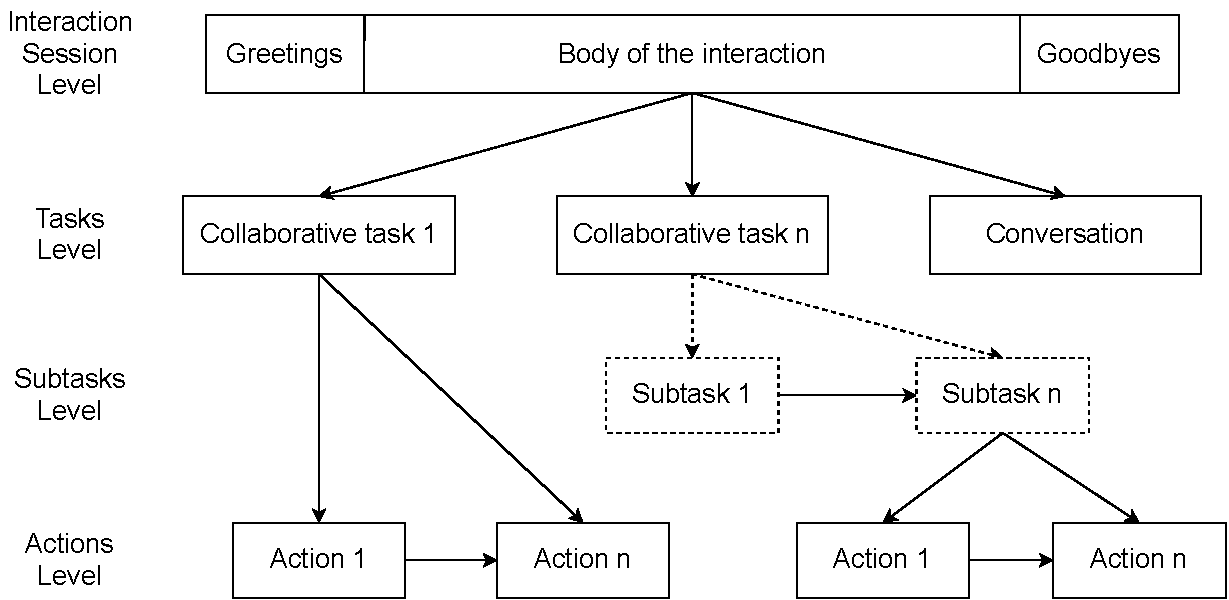
\includegraphics[width=\linewidth]{figures/chapter2/session_interaction.pdf}
	\caption{The hierarchical structure of an interaction session. The highest level is the interaction session. The second level is composed of the tasks. They are included in the body of interaction of the interaction session and, two types of tasks are considered and may overlap, collaborative and conversational tasks. With this representation, a task can be recursively refined as subtasks until reaching the last level, the actions level, which is considered as atomic.
%		Subtasks are not considered as a ``real'' level of the interaction session, specially to evaluate the \acrshort{qoi}, as it may exist or not according to the task.
		}
	\label{fig:levels}
\end{figure}


\subsection{Representation of a Human-Robot Interaction Session}
We define an \textbf{interaction session} as the period during which the robot and a human interact together and are engaged. It is divided in three parts, following the structure proposed by Robinson~\cite{robinson_overall_2012} as presented in Section~\ref{chap2:sec:soc_inter}: the greetings, the body of the interaction and the goodbyes. First, \textit{the greetings} corresponds to the period where an agent starts an interaction by initiating it with another agent. The interaction session lasts as long as the interactants are maintaining the interaction through conversation and collaborative tasks performance which corresponds to the \textit{body of interaction}. Finally it ends when at least one of the interactants is disengaged, either by abruptly ending the interaction or by closing the interaction as described by Schegloff and Sacks~\cite{schegloff_1973_opening}, it corresponds to ``the goodbyes''. For example, for an entertainment robot in a mall, an \textit{interaction session} starts when a person signals to the robot that they want to engaged, by greeting it or by approaching it and looking at it. The body of interaction is composed of conversation and eventually direction-giving tasks and, the session lasts until the person says goodbye or leaves. This is the nominal case and, the duty of the robot is to contribute to maintain the session alive until the human decides to close it, because it is at the service of humans. However, in some (extreme) cases, the robot might decide to close the interaction by itself.

Moreover, as seen in Section~\ref{chap1:subsubsec:joint_commit}, social interactions and joint activities (or actions) involve commitment, or rather engagement as we say in robotics -- this difference in the vocabulary as been highlighted in~\cite{castro_2019_commitments}. As explained in the previous chapter, there is no unique definition of what it means to be engaged. We chose one that is frequently used in robotics, proposed by Sidner and Lee~\cite{sidner_2003_engagement}: ``Engagement is the process by which two (or more) participants establish, maintain and end their perceived connection during interactions they jointly undertake''. The robot must be able to exhibit its engagement and disengagement and also to assess them with respect to its human partner.

We defined three states for the body of interaction, corresponding to what can happen during the latter: 
\begin{bulletList}
	\item conversation: a social chit-chat or a goal negotiation, without any physical action performed except communicative gestures
	\item collaborative task: both agents executing actions in order to achieve a shared goal
	\item idle phases: the agents are not chatting or performing a collaborative task together but remain engaged in the interaction session, it happens in-between active interaction phases
\end{bulletList}

For each of these three states, the way to exhibit the engagement varies (\eg in a conversation, an agent looking at their partner displays their engagement; during a task, an agent correctly performing their action is a way to demonstrate their engagement). That is why there is a need to define what behavior the robot has to exhibit in each state and what behavior it should expect from the human in each state, as these behaviors are usually very specific (\eg in a direction-giving task, the robot keeps its head oriented toward its partner's face to demonstrate its engagement in conversation and idle contexts and when it gives a direction it expects the human to look at the direction it is showing; in a stack task, when the robot gives an instruction it expects the human to take a given cube).

Transitions from one state to another can be managed by triggers more or less complex. For example, a collaborative task can be initiated when a human asks the robot that they achieve a goal together.


\subsection{Collaborative Tasks, Substasks and Actions}
\textbf{\textit{Tasks}} compose the body of the interaction of an interaction session as shown in Fig.~\ref{fig:levels}. We distinguish conversation (\ie agents engage in dialogue to exchange ideas, or to ask questions) from collaborative tasks (\ie agents work as partners, collaborating to perform tasks and to achieve common goals). We will not develop more on conversation since it is not the main focus of this work.

In joint or collaborative activities (see Section~\ref{chap1:subsec:def_ja}), humans are committed to achieve a goal together, involving collaboration and shared plans as shown in Section~\ref{chap1:sec:ja}. And, when interaction with a robot, the same mechanisms are also triggered as they are essential to a successful collaboration. When a human and a robot perform a task together, as described by Bauer \textit{et al}.~\cite{bauer_2008_collab}, we could say that the robot has the intent to help the human, so the human's intention becomes its own intention. Then, they have the joint intention to reach a common goal and, as shown by Michael and Salice~\cite{michael_2017_commitment}, they have a commitment to the joint activity, leading to perform joint actions. Therefore, during its evaluation and decision-making processes, the robot has to take into account that the human and itself should remain engaged all along an interaction session for the tasks to be successful and both have to manage and contribute to maintain expectations about what the other is doing. 

The elements composing a \textit{task} are: a goal, a plan and involved agents. A plan is needed to achieve a goal. The ones we manipulate are \acrshort{htn}-based plans, composed of \emph{abstract tasks} that we also call \emph{subtasks} and \emph{primitive tasks} that we also call \emph{actions}.

\textbf{\textit{Actions}} are the elementary items of tasks, \emph{primitive tasks}, manipulated by the high-level robot supervision controller. They cannot be decomposed further by it (\eg placement and motion planning are achieved by a lower control system not described here). It is usual to describe an action with its preconditions, its effects and, the agents and entities implied in its execution (\eg in plans written in PDDL (Planning Domain Definition Language)~\cite{ghallab_98_pddl}). We add to this description the notion of expected reactions (which can themselves be actions) from the other agents once the action is executed.

In our model, an agent (human or robot) is a contributor to the task and has a mental state as described by Devin \textit{et al}.~\cite{devin_2016_implemented}. The mental state is a set of facts representing, from the agent point of view, the current world state, the state of the goal and the current task state. Since we are interested here in the robot situation assessment and decisional processes, the mental state of the human is built and managed by the robot as an estimation of the beliefs of the human~\cite{milliez_2014_framework, hiatt_2017_modeling,tabrez_2020}.

\section{The Structure of JAHRVIS}\label{chap5:sec:jahrvis}
%\section{The Architecture of JAHRVIS}\label{chap5:sec:jahrvis}
The \acrfull{jahrvis} is implemented on top of our ROS-Jason framework\footnote{\url{https://github.com/amdia/ld_rjs}}. During the design of \acrshort{jahrvis}, we identified seven high-level features we needed and implemented their associated processes, based on the objectives presented in Section~\ref{chap5:sec:sup_features}\footnote{The design of \acrshort{jahrvis} was an iterative work, indeed the first version being the supervisor implemented for the task described in Chapter~\ref{chapter:chap8}, the second one was the supervisor of the task described in Chapter~\ref{chapter:chap9} and the final one was the supervisor of the example used all along Chapter~\ref{chapter:chap6}}. We present \acrshort{jahrvis} structure in Figure~\ref{chap5:fig:sup_overview}, with the seven processes in blue, the \acrshort{qoi} Evaluator dedicated to the interaction evaluation and the six others to the decision and control. All the next developments of this chapter will be about the description of these processes. The components not in blue are external components from the robotic architecture presented in Section~\ref{chap3:sec:rob_archi} to which a part of knowledge maintenance, decision-making and execution are delegated by \acrshort{jahrvis}.

\begin{figure}[!ht]
	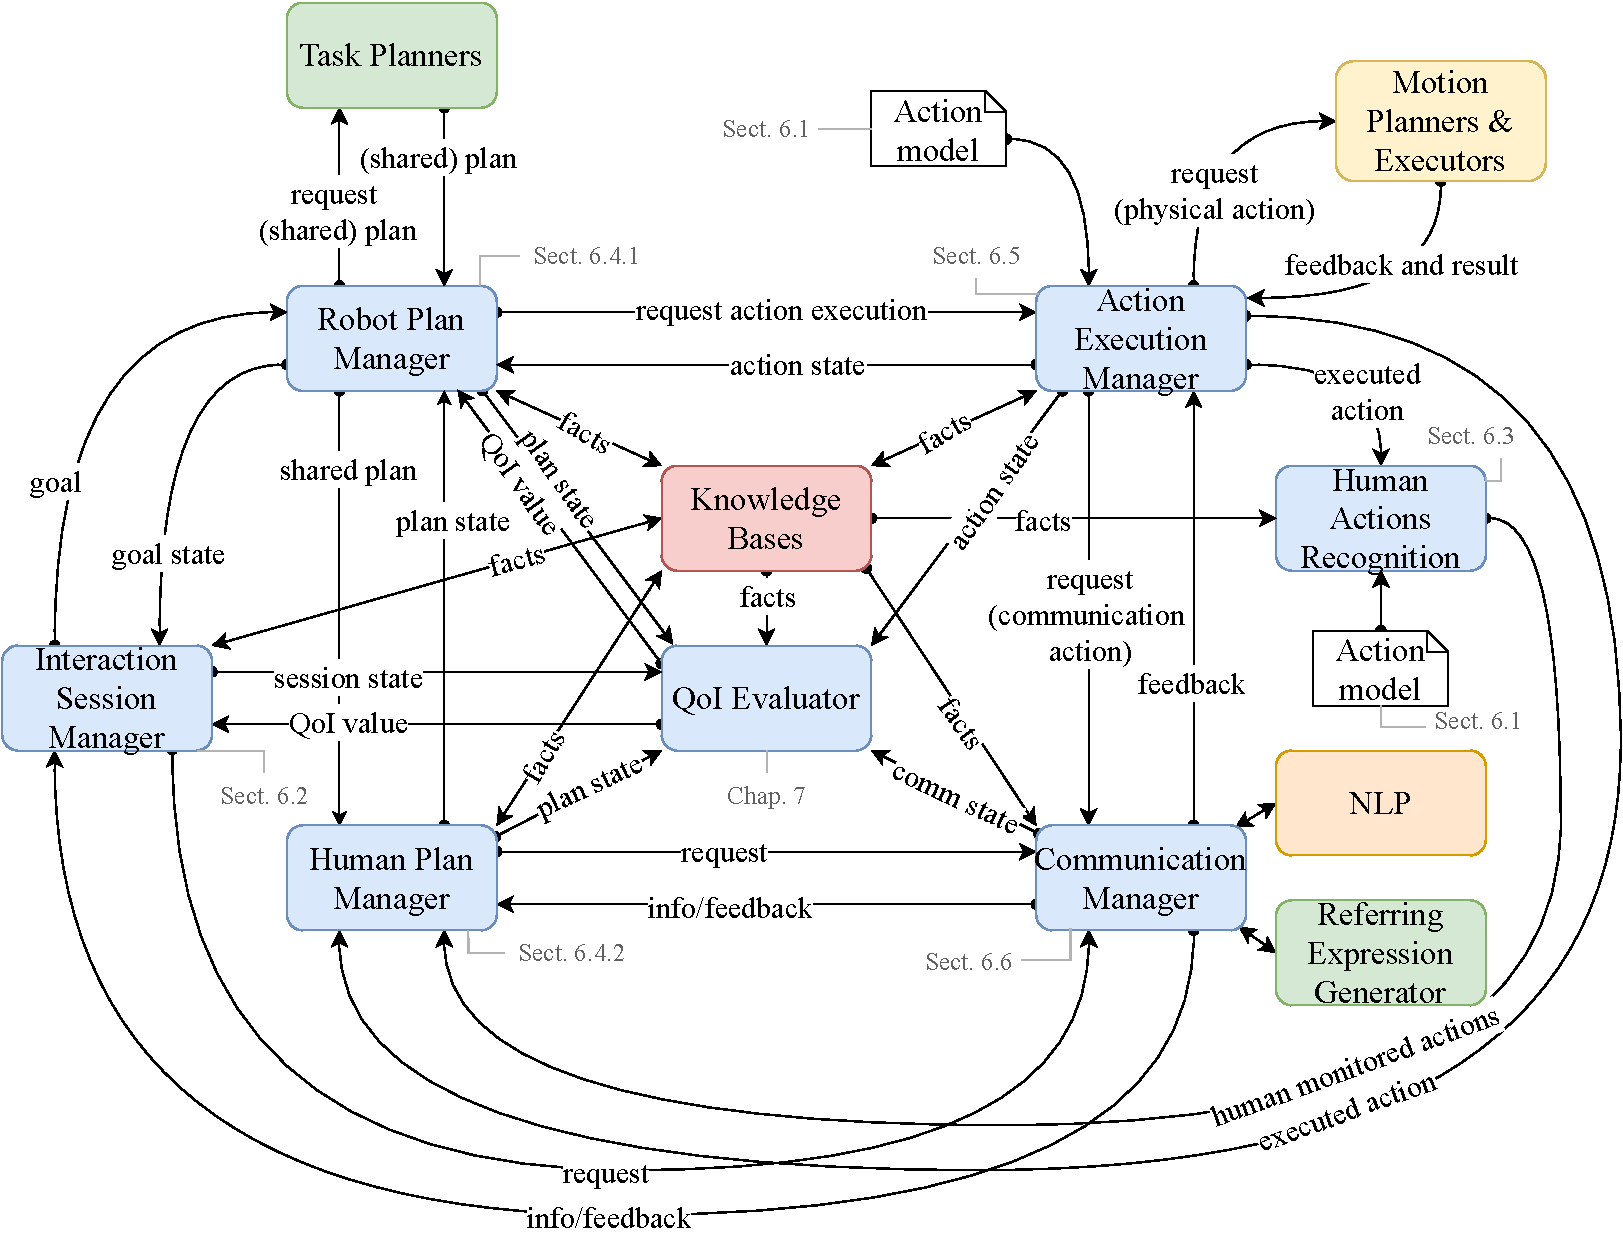
\includegraphics[width=\linewidth]{figures/chapter2/supervisor_modules.pdf}
	\caption{The \acrshort{jahrvis} processes (in blue) and their interactions between themselves and with the other components of the robotic architecture presented in Section~\ref{chap3:sec:rob_archi}.}
	\label{chap5:fig:sup_overview}
\end{figure}\todo{update section numbers}

For each process (in blue in Figure~\ref{chap5:fig:sup_overview}), we implemented a \acrfull{rja}, with the desired behavior coded in ASL and the needed customizations added in Java. Thus, internal communications between the \acrshort{jahrvis} processes, and so \acrshort{rja}s, use Jason messages (see Section~\ref{chap4:subsec:jason}). External communication with the other components of the robotic architecture is based on either ROS messages, services or action clients.

Not all \acrshort{rja}s are active at each level of interaction defined in Section~\ref{chap5:sec:levels}. Indeed, as its name suggests, the \textit{Interaction Session Manager} handles interaction sessions. The \textit{Robot} and \textit{Human Plan Managers} handle the task level. And, the \textit{Action Execution Manager} and the \textit{\acrlong{ham}} are in charge of the action level. The \textit{Communication Manager} is active at all levels. We can also make the distinction between the component dedicated to the assessment of the quality of interaction, \ie the \acrshort{qoi} Evaluator which will be described in Chapter~\ref{chapter:chap7}, and all the other ones, dedicated to the decision-making and control.

Figure~\ref{chap5:fig:data_state} shows an overview of the data representing the state of \acrshort{jahrvis} at each instant when the system runs. The robot can either be in an interaction session with a human or be by itself. When it is in an interaction session, it computes the human's commitment (it may be a simple function checking if the human is here or not) and is available to perform collaborative tasks. When the robot is not interacting with humans, it can have tasks to perform such as going to its home base. If a collaborative task should start (on human request or on the robot's initiative), a (shared) plan is got from the Task Planner as shown in Figure~\ref{chap5:fig:sup_overview}. When the collaborative task is ongoing, the robot has its beliefs about the environment and the plan progress, and estimates the human's ones. Beliefs about the environment are provided by other components of the robotic architecture presented in Section~\ref{chap3:sec:rob_archi}: the Situation Assessment and the Knowledge Bases. Each abstract and primitive task has a number of data associated to it. Moreover, \acrlong{qoi} and human action recognition are continuously processed. Finally, when an action is executed by the Motion Planners and Executors, updates about the action states are communicated to \acrshort{jahrvis}.

\begin{figure}[!ht]
	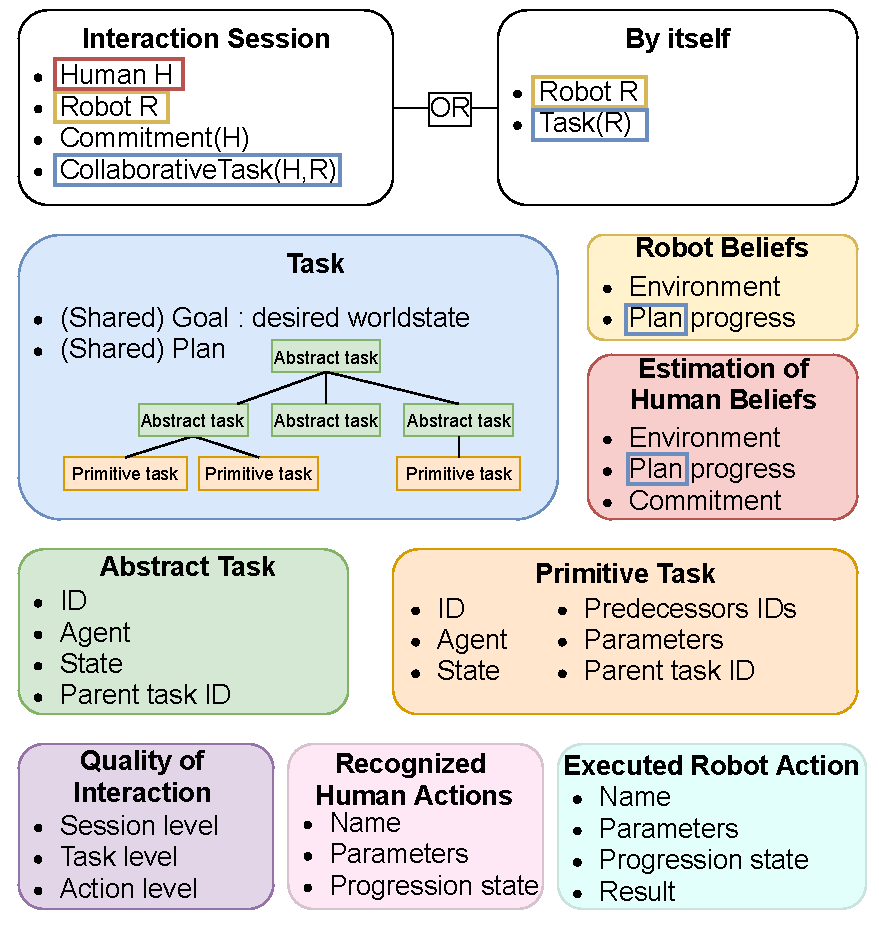
\includegraphics[width=\linewidth]{figures/chapter2/data_state_representation.pdf}
	\caption{Overview of the data representing the state of \acrshort{jahrvis} at each instant when the system runs. The robot can either be in an interaction session with a human or be by itself. When it is in a task, plan progress are maintained from the robot's and human's estimated point of views. A plan is composed of abstract and primitive tasks whose state evolved during the task. \acrshort{qoi} and human action recognition are two elements continuously computed. When the robot executes an action, the state of the later is updated as well as its result (success or failure).}
	\label{chap5:fig:data_state}
\end{figure}

In the Chapters~\ref{chapter:chap6} and \ref{chapter:chap7} will be presented these processes. Chapter~\ref{chapter:chap6} introduces the ones related to the decision-making and robot control while Chapter~\ref{chapter:chap7} describe the evaluation process of the \acrlong{qoi}. Chapter~\ref{chapter:chap6} will start by laying the foundations for the \acrshort{rja} functioning: the knowledge representations and management. Then, each \acrshort{rja} will be thoroughly described. The \acrfull{ism} is dedicated to in-between tasks, \ie the opening and closing of interactions and all the dialog which can happen between two collaborative tasks. When a shared goal is established, the shared plan is handled by the \acrfull{rpm} and the \acrfull{hpm}, \ie to follow the plan progression, to make sure that the observed human actions match the ones of the plan and to decide when the robot should act. Robot actions to perform are sent to the \acrfull{aem} that interfaces with the motion planers and executors. As for human actions, they are monitored and recognized by the \acrfull{ham}. Finally, the \acrfull{cm} is in charge of producing the communication for the human when requested by another \acrshort{rja} along with the human communication reception.




\ifdefined\included
\else
\bibliographystyle{acm}
\bibliography{These}
\end{document}
\fi






